\documentclass[a4paper,12pt]{report}
\linespread{1.5}
\usepackage{geometry}
\geometry{top=3cm,bottom=3cm,left=3.5cm,right=3.5cm} % Impostiamo il valore dei margini.
\usepackage[utf8]{inputenc}
\usepackage{tikz,pgf}
\usepackage{indentfirst}
\usepackage{amsfonts}
\usepackage[english]{babel} %% Abbiamo istruito LaTeX ad usare la lingua italiana.
\usepackage{todonotes}
\usepackage{subfig}
\usepackage{fancyhdr}
\setlength{\parindent}{1cm}
\usepackage{graphicx}
\usepackage{longtable}
\usepackage{csquotes}
\usepackage{amsmath}
\usepackage{numprint}
\usepackage{pgfplots}
\usepackage{pgfplotstable}
\usepackage{tocbibind}
\usepackage{titling}
\usepackage{wrapfig}
\usepackage{graphics}
\usepackage[bookmarksopen,bookmarksdepth=2,breaklinks=true,colorlinks=true,urlcolor=black,linkcolor=black]{hyperref}
\graphicspath{{imgs/}} %% cartella dalla quale ricavare le immagini %%
\usepackage{booktabs}
\usepackage{float}


\setlength {\marginparwidth }{2cm} 
\pgfplotsset{compat=1.16}

\newenvironment{dedication}
  {\clearpage           % we want a new page
   \thispagestyle{empty}% no header and footer
   \vspace*{\stretch{1}}% some space at the top 
   \itshape             % the text is in italics
   \raggedleft          % flush to the right margin
  }
   {\par % end the paragraph
   \vspace{\stretch{3}} % space at bottom is three times that at the top
   \clearpage           % finish off the page
  }
  

\begin{document}
\begin{titlepage}
\begin{center}
\textbf{\LARGE University of Calabria}\\
\textbf{Dipartimento di Ingegneria Informatica, Modellistica, Elettronica e Sistemistica - DIMES}\\
\vskip 6pt
\hrule
\vskip 8pt
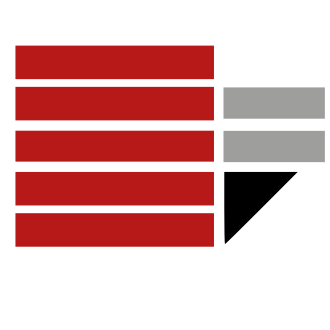
\includegraphics[width=0.13\linewidth]{logo.png}
\vskip 8pt
\textbf{Master’s degree course in Computer Engineering for the Internet of Things}
\vskip 32pt
Big Data Analystics

\vskip 70pt
{ \huge \bfseries 
Income Predict and Customer Clustering
}\\[0.4cm]
\vskip 7pt

\vskip 100pt

\begin{tabular}{p{8cm}p{6cm}}
Respective Faculty: & Authors:\\
Prof.~Andrea Tagarelli & Wang Hongyu 225200 \\
Prof.ssa Lucio La Cava & Yang Qing xxxxxx \\
 & Najeebullah Shirzad
 xxxxxx \\

\end{tabular}

%\begin{tabular}{p{8cm}p{8cm}}
%\includegraphics[width=0.3\linewidth]{imgs/firma.jpg}
%&
%\includegraphics[width=0.3\linewidth]{imgs/firma.jpg}
%\end{tabular}

\vskip 60pt
\hrule
\vskip 6pt
Anno Accademico 2022/2023
\vfill
\end{center}

\end{titlepage}

\begin{dedication}
Namaste
\end{dedication}

%% Corpo della tesi %%

%\chapter*{Sommario} %% In questa zona inseriamo l'abstract del nostro documento. %%
%Inserisci abstract: ...



\tableofcontents
\newpage
\chapter{Business Understanding And Data Understanding}
\section{Business Understanding}

According to the dataset, predicting customer income can provide better benefits to the company. By clustering customers, it is possible to analyze their behavior and gain insights into their preferences and needs. This can help companies tailor their products and services to meet the specific needs of their customers. Such an approach can lead to increased customer satisfaction and loyalty, which can ultimately translate into higher profits for the company. 

\subsection{Data mining Goals}
%(Describe the intended outputs that enables the achievement of the project objectives) 
The goal is to create a tool capable of estimating new properties that will be put on the market, understanding the importance of the parameters that contribute to the economic evaluation of the property, in order to have a more accurate estimate of the value of the property based on the parameters that allow its value to be surveyed. For each property there is no right or wrong answer to its market value and it is not even possible to make a comparison with other properties present, albeit close to rent, as each property has different characteristics from each other.

\subsection{Data mining Success Criteria}
%(Define the criteria for a successful outcome) 
The success criteria should be based on the data mining goal determined earlier and should be used to formulate benchmarks for success. The methods for model assessment should be described, and benchmarks for evaluating success should be defined. Specific numbers should be provided, and subjective measurements should be determined as best as possible. 

The phases that we are going to perform by dividing the work by trying different methodologies in order to create a model as close as possible to the training set provided.
The distributing the hours in this way:
\begin{itemize}
\item Business Understanding: 5\% of total hours;
\item Data Understanding: 10\%;
\item Data Preparation: 60\%; 
\item Modeling: 20\%;
\item Evaluation: 5\%.
\end{itemize}

\subsection{Data Description Report}
% Describe the data that has been acquired including its format, its quantity

The dataset has the following characteristics: 
\begin{itemize}
    \item Multivariate;
    \item 2240 rows representing the number of records;
    \item 29 columns representing the number of attributes in the dataset;
\end{itemize}

The details of the dataset can be found at   

\href{kaggle}{https://www.kaggle.com/datasets/rodsaldanha/arketing-campaign}


\input{capitoli/capitolo2}
\chapter{Data Preparation}

\section{Data Cleaning}

\subsection{Missing Value}
% List the data to be included/excluded and the reasons for these decisions
Missing values are quite common in many real-life datasets. There are different ways of handling missing values with dataset examples.
With this dataset, there is only one attribute with missing values and there are only a limited number of instances, then replaced this the rows with mean values is a reasonable approach.
the method we used in weka is \textit{weka.filters.unsupervised.attribute.ReplaceMissingValues}
Here is the detail of the Attribute Income which contains missing value.
\begin{itemize}
    \item \textbf{Income} 24 instance of missing value, 1\% to the total insstance;
\end{itemize}


\subsection{Remove Outlier}
For this dataset there do existing some attribute which containing the Outlier, we use the method of \textit{weka.filters.unsupervised.attribute.InterquartileRange} to find out the Outliers of each attribute.
After executing the method \textit{weka.filters.unsupervised.instance.RemoveWithValues} to remove the redundant value, two more attributes will be added which shows the Outliers and ExtremeValue. 

\section{Discretization}
Discretization is the process of transferring continuous functions, models, variables, and equations into discrete counterparts.  
In weka, there is a method \textit{weka.filters.unsupervised.attribute.Discretize} transform continuous variables into discrete ones. Discretization can also help to reduce the dimensionality of the data and improve the performance of some machine learning algorithms.

\section{Sampling}
Data sampling provides a collection of techniques that transform a training dataset in order to balance or better balance the class distribution.
In this case, we sampling a balanced dataset accroding to the minimun number of Income attribute. After balancing the dataset, there have 650 insstance of each label for Income.
\section{Dimensionality Reduction}
Dimensionality reduction is a technique of reducing the number of input variables or features in a dataset. It aims to obtain a set of principal or lower-dimensional variables that capture the essence or structure of the data.
\subsection{Eliminate irrelevant}

\begin{itemize}
    \item \textbf{Dt\_Customer}: After modifying the attribute Dt\_Customer to the uniform format and putting it into the model, the model did not perform well in the processing phase for both clustering and classification. However, when it was deleted from the features, the performance of the task improved.
    \item \textbf{ID}: The ID is irrelevant to the training process.
    \item \textbf{Z\_CostContact}: All items are the same.
    \item \textbf{Z\_Revenue}: All items are the same.
    \item \textbf{Complain}: The attribute contains little entropy.
\end{itemize}

There also some more attributes which record the customer accepted the offer in the campaign. These attributes were removed from the clustering task because they contained less entropy. After removing these features, the performance of clustering algorithms improved.
\begin{itemize}
    \item \textbf{AcceptedCmp1}; \textbf{AcceptedCmp2}; \textbf{AcceptedCmp3} \textbf{AcceptedCmp4}; \textbf{AcceptedCmp5}
\end{itemize}

\section{Feature Creation}
Using the method \textit{weka.filters.unsupervised.attribute.Discretize} that discretizes a range of numeric attribute, the attributes which used the method are listed bellow.
\begin{itemize}
    \item \textbf{Year\_Birth}: the year of birth are splite into three nominal attributes.
    \item \textbf{Income}: the Income are splite into three nominal attributes also as the classification label.
\end{itemize}


\section{Attribute Transformation}
The mothod of \textit{weka.filters.unsupervised.attribute.OrdinalToNumeric} is an attribute filter that converts ordinal nominal attributes into numeric ones. This operator not only changes the type of selected attributes but it also maps all values of these attributes to numeric values. 
After the operation of OrdinalToNumeric, this will allow for the use of numerical algorithms such as those presented in the Numerical Algorithms


\chapter{Modeling And Evaluation}

\section{Select Modeling Tecnique}

\subsection{Modeling Technique for Classification}
% Document the modeling technique that you’ll be using
Random Forest Tree: Random forest is an ensemble learning method for classification, regression and other tasks that operate by constructing a multitude of decision trees at training time and outputting the class that is the mode of the classes (classification) or mean prediction (regression) of the individual trees. Random forest is known for its accuracy and robustness to noise and outliers.

Naive Bayes: Naive Bayes is a probabilistic algorithm that is based on Bayes’ theorem. Naive Bayes is used for classification problems and is known for its simplicity and speed.

Decision Tree: A decision tree is a supervised learning algorithm that is used for classification and regression modeling. It is a method used for predictive modeling, so these trees are used to either classify data or predict what will come next. Decision trees in machine learning can either be classification trees or regression trees. 

\subsection{Modeling Technique for Clustering}

Bisecting K-means: Bisecting K-means is a hierarchical clustering algorithm that recursively bisects clusters until the desired number of clusters is reached. The algorithm starts with all data points in one cluster and then splits the cluster into two smaller clusters. The splitting is done by running K-means on the larger cluster and splitting it into two smaller clusters based on the K-means output. The process is repeated until the desired number of clusters is reached.

K-means: K-means is a clustering algorithm that partitions n observations into k clusters in which each observation belongs to the cluster with the nearest mean. The algorithm starts by randomly selecting k initial centroids. Each observation is then assigned to the nearest centroid. The mean of each cluster is then calculated and used as the new centroid. This process is repeated until the centroids no longer change or a maximum number of iterations is reached.

Gaussion Mixture: Gaussian Mixture Model (GMM) is a probabilistic model that assumes that the data is generated from a mixture of several Gaussian distributions with unknown parameters. The algorithm starts by randomly initializing the parameters of the Gaussian distributions. The expectation-maximization (EM) algorithm is then used to estimate the parameters of the Gaussian distributions. The EM algorithm iteratively estimates the parameters of the Gaussian distributions until convergence. 

\subsection{Modeling Assumptions}
% Record any assumptions about the data that are necessary for the modeling techniques
Random Forest Tree: Random forest assumes that the data is independent and identically distributed (i.i.d.) and that there are no missing values in the data.

Naive Bayes: Naive Bayes assumes that the features are independent of each other and that there are no missing values in the data.

Decision Tree: Decision tree is a non-statistical approach that makes no assumptions of the training data or prediction residuals; e.g., no distributional, independence, or constant variance assumptions.

Bisecting K-means: Bisecting K-means makes no assumptions about the underlying data distribution 

K-means:The variance of the distribution of each attribute (variable) is spherical and all variables have the same variance.

Gaussian mixture models: Gaussian mixture models (GMMs) are a probabilistic model that assumes all the data points are generated from a mixture of a finite number of Gaussian distributions with unknown parameters

\section{Build Model And Evaluation}  

We used the \textit{org.apache.spark.ml} library for the training process. There also employed 5-fold cross-validation to train the model and select the best model for evaluation.
\subsection{Random Forest Tree}

After Modeling the result of Confusion Matrix~\ref*{cmRFT} and evaluation table~\ref*{tableRFT} list here.


\begin{table}[H]  \centering  
    \begin{tabular}{@{}lllll@{}}
    \toprule
    \multicolumn{5}{c}{Random Forest Tree}                 \\ \midrule
    \multicolumn{5}{l}{Accuracy: 0.9775641025641025}       \\\midrule
                 & precision & recall & f1-score & FPR \\
    0.0         & 0.97      & 0.99   & 0.98     & 0.01      \\ 
    1.0          & 0.98      & 0.93   & 0.96     & 0.00     \\
    2.0       & 0.97      & 1.00   & 0.98     & 0.01     \\
    
    Weighted precision    & \multicolumn{4}{c}{0.977800279509976}         \\
    Weighted recall    & \multicolumn{4}{c}{0.977564102564102}          \\
    Weighted F1 score    & \multicolumn{4}{c}{0.977369021913490}        \\
    Weighted false positive rate & \multicolumn{4}{c}{0.011880522633986}         \\ \bottomrule
    \end{tabular}
    \caption{Classification Report of Random Forest}
    \label{tableRFT}
\end{table}





\begin{figure}[H]
    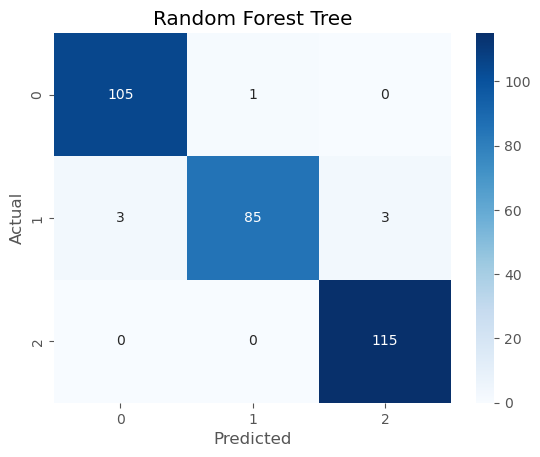
\includegraphics[scale=0.7]{imgs/rft}
    \centering
    \caption{Confusion Matrix of Random Forest Tree}
    \label{cmRFT}
\end{figure}


\subsection{Naive Bayes}

As for the Naive Bayes, the result of Confusion Matrix~\ref*{cmnb} and evaluation table~\ref*{tablenb} list here.


\begin{table}[H]\centering
    \begin{tabular}{@{}lllll@{}}
    \toprule
    \multicolumn{5}{c}{Naive Bayes}                 \\ \midrule
    \multicolumn{5}{l}{Accuracy: 0.7852564102564102}       \\\midrule
                 & precision & recall & f1-score & FPR \\
    0.0         & 0.78      & 0.95   & 0.84     & 0.16      \\ 
    1.0          & 0.70      & 0.45   & 0.55     & 0.07     \\
    2.0       & 0.85      & 0.89   & 0.87     & 0.08     \\
    
    Weighted precision    & \multicolumn{4}{c}{0.7786264164368255}         \\
    Weighted recall    & \multicolumn{4}{c}{0.7852564102564104}          \\
    Weighted F1 score    & \multicolumn{4}{c}{0.7695695968516545}        \\
    Weighted false positive rate & \multicolumn{4}{c}{0.1086680781804235}  \\ \bottomrule
    \end{tabular}
    \caption{Classification Report of Naive Bayes}
    \label{tablenb}
    \end{table}

\begin{figure}[H]
    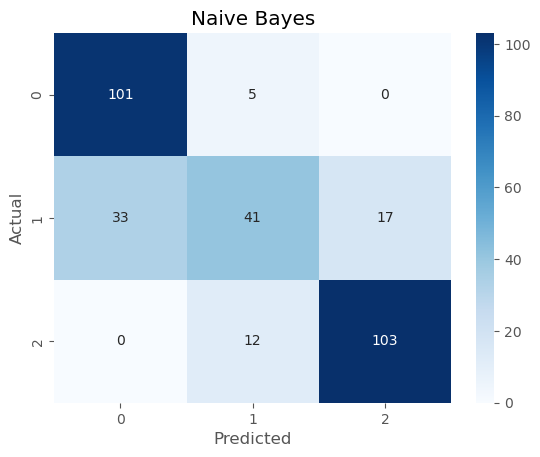
\includegraphics[scale=0.7]{imgs/nb}
    \centering
    \caption{Confusion Matrix of Naive Bayes}
    \label{cmnb}
\end{figure}

\subsection{Decision Tree} 

The DecisionTreeClassifier is a class in the sklearn.tree module of the Python Scikit-learn library. It is used to create a decision tree classifier which is a predictive model that can be used for both classification and regression problems. The criterion parameter specifies the function to measure the quality of a split. In this case, we use the supported criteria is “gini” for the Gini impurity.
Confusion Matrix~\ref{cmdt} and Classification Report of Decision Tree~\ref{tabledt}.
\begin{table}[H]\centering
    \begin{tabular}{@{}lllll@{}}
    \toprule
    \multicolumn{5}{c}{Decision Tree}                 \\ \midrule
    \multicolumn{5}{l}{Accuracy: 0.8269230769230769}       \\\midrule
                 & precision & recall & f1-score & FPR \\
    0.0         & 0.84      & 0.90   & 0.82     & 0.08      \\ 
    1.0          & 0.71      & 0.67   & 0.69     & 0.10     \\
    2.0       & 0.89      & 0.87   & 0.88     & 0.06     \\
    
    Weighted precision    & \multicolumn{4}{c}{0.8248610604716251}         \\
    Weighted recall    & \multicolumn{4}{c}{0.8269230769230769}          \\
    Weighted F1 score    & \multicolumn{4}{c}{0.8252391066535802}        \\
    Weighted false positive rate & \multicolumn{4}{c}{0.0838127083514056}  \\ \bottomrule
    \end{tabular}
    \caption{Classification Report of Decision Tree}
    \label{tabledt}
    \end{table}

    \begin{figure}[H]
        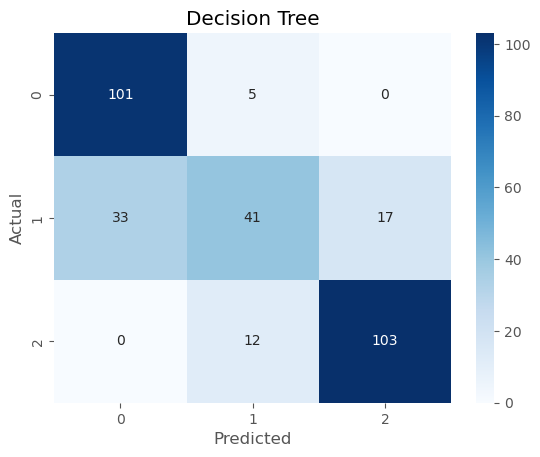
\includegraphics[scale=0.7]{imgs/dc}
        \centering
        \caption{Confusion Matrix of Decision Tree}
        \label{cmdt}
    \end{figure}

\subsection{Clustering Task}

The Silhouette method is a way to evaluate the quality of clustering. It measures how similar an object is to its own cluster compared to other clusters. The Silhouette score ranges from -1 to 1. A score of 1 indicates that the object is well matched to its own cluster and poorly matched to neighboring clusters.
the table\ref{cluster} show the performance of each algorithms.
\begin{table}[]
    \begin{tabular}{ll}
    \hline
    \multicolumn{2}{c}{Cluster Task}                                                     \\ \hline
                        & \multicolumn{1}{c}{Silhouette with squared euclidean distance} \\
    K means             & 0.2185969767629818                                             \\
    Gaussian Mixture    & 0.2139769508957303                                             \\
    Biselecting K-means & 0.3698272179197341     \\ \bottomrule
    \end{tabular}
    \caption{Evaluation of Cluster}
    \label{cluster}    
    \end{table}
\chapter{Knowledge}

In this chapter, we will list some interesting phenomena that were obtained from the cluster modeling process.

\section{Feature comparation}



\begin{figure}[H]
  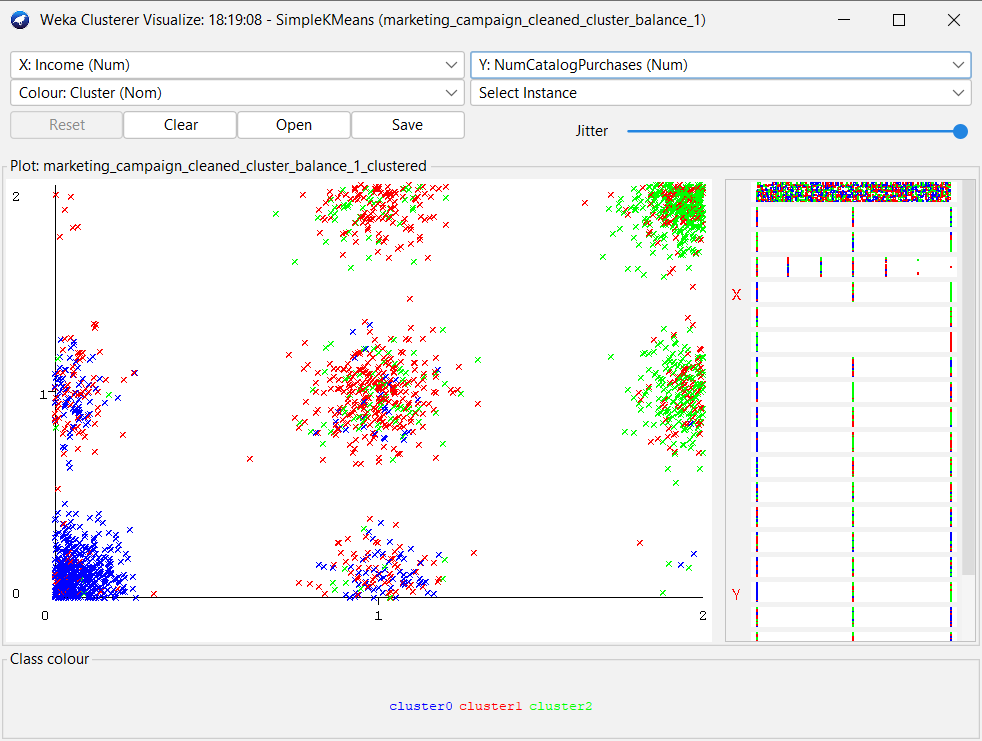
\includegraphics[scale=0.6]{imgs/cluster_income_catalog}
  \centering
  \caption{Income - NumCatalogPurchases}
  \label{NumCatalogPurchases}
\end{figure}

The figure\ref{NumCatalogPurchases} displays the distribution of income and the number of purchases made using catalogues. It appears that individuals with higher income tend to use catalogues to make purchases, while those with lower income tend to do the opposite.


\begin{figure}[H]
  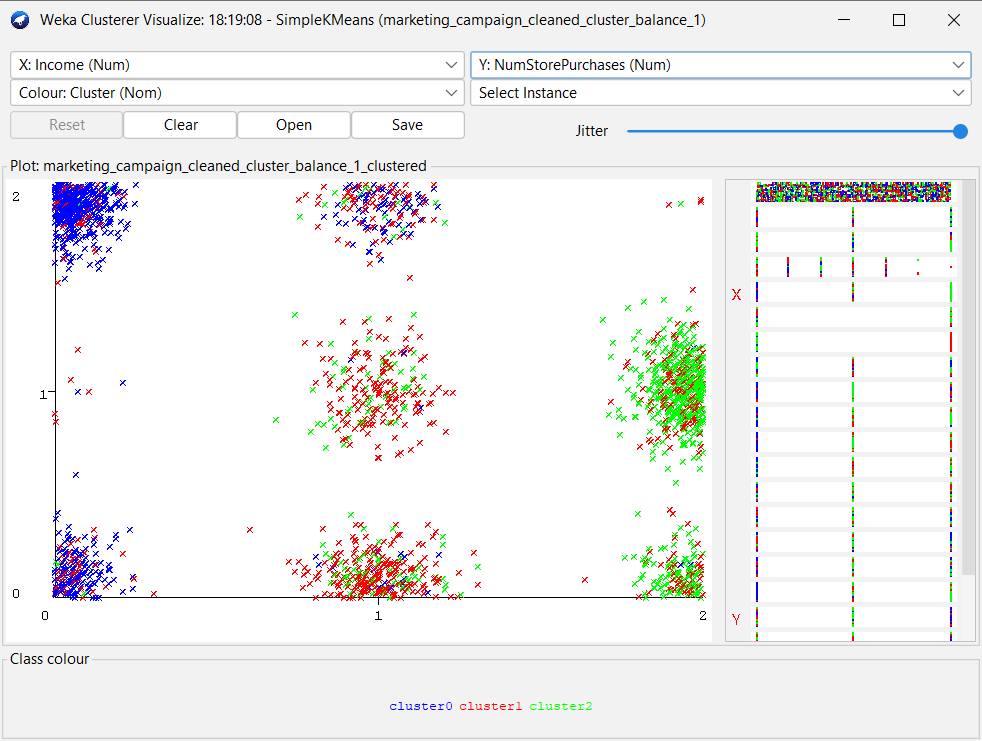
\includegraphics[scale=0.6]{imgs/cluster_income_store}
  \centering
  \caption{Income - NumStorePurchases}
  \label{NumStorePurchases}
\end{figure}

The figure\ref{NumStorePurchases} indicates that individuals with lower income tend to prefer purchasing items from stores, while those with higher income tend to make fewer purchases from stores.



\begin{figure}[H]
  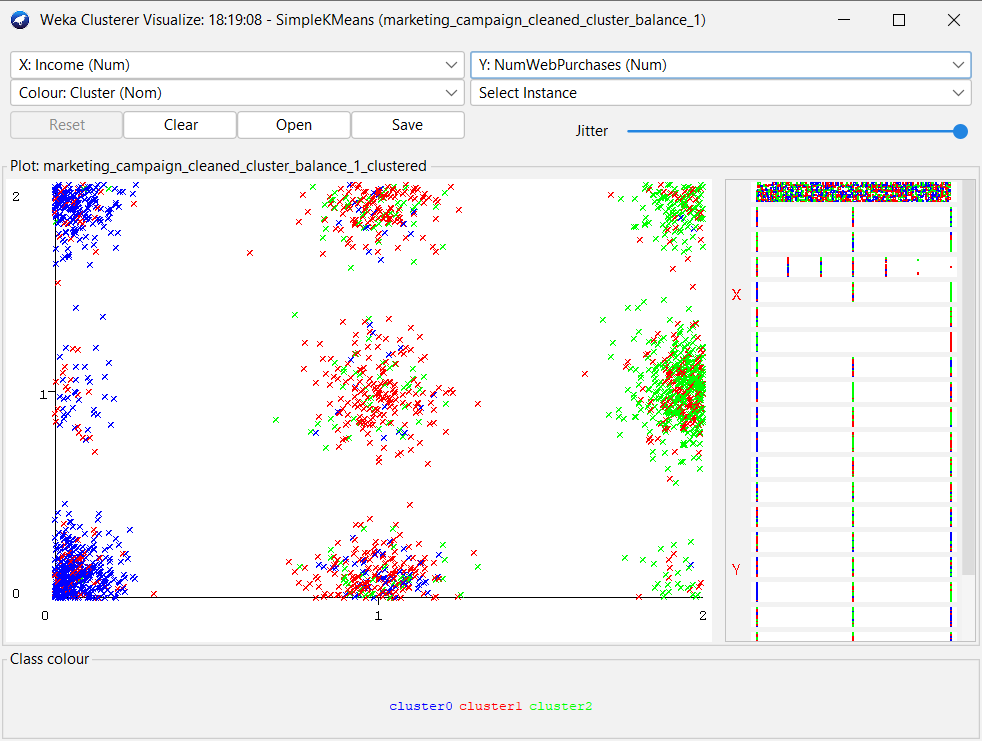
\includegraphics[scale=0.6]{imgs/cluster_income_webbuy}
  \centering
  \caption{Income - NumWebPurchases}
  \label{NumWebPurchases}
\end{figure}

The figure\ref{NumWebPurchases} shows that there are two extreme groups of lower Income: one that prefers to buy a great amount of items online and the other that does not. For the higher income class, most individuals prefer buying items online.

\begin{figure}[H]
  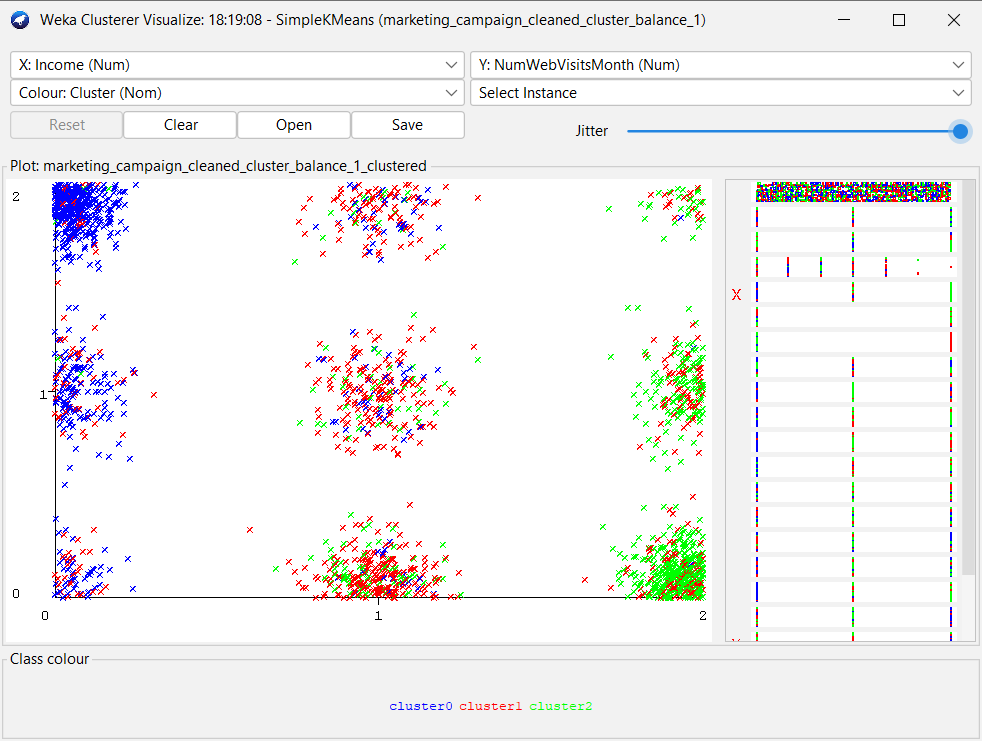
\includegraphics[scale=0.6]{imgs/cluster_income_webvisit}
  \centering
  \caption{Income - number of visits to company’s web site}
  \label{VisitPermonths}
\end{figure}

The figure\ref{NumWebPurchases}, it appears that individuals with lower income tend to visit a greater amount of stores, while those with higher income tend to do the opposite.
%\chapter{Bibliografia}

%[1] Android Developers. \\
%URL: \url{https://developer.android.com}\\

%Eliminare/Aggiungere/Personalizzare i capitolo nella cartella "capitoli"

%\chapter*{Conclusioni} In questo modo non comparirà dell'indice

%\begin{thebibliography}{100} %% 100 rappresenta il n° massimo di voci all'interno della bibliografia: può essere modificato a vostro piacimento. %%
%\bibitem{[1]:}
%\bibitem{[2]:}
%\bibitem{[3]:}
%\bibitem{[4]:}

%\end{thebibliography}

%\chapter*{Ringraziamenti}
%Inserisci frasi sdolcinate: ...
\end{document}
